\chapter{Problem Formulation}
\label{chap:Problem_Formulation}

To test our hypothesis for the \acs{parlpo} framework, we propose a constrained zero-sum game, based on linear-time-invariant 2nd-order \acs{hcw} dynamics (or linear time-varying elliptic dynamics) to model the interaction of two agents relative to a chief circular orbit in the Local-Vertical Local-Horizontal (\acs{lvlh}) frame. We bound these agents into an imaginary spherical arena in space centered at the chief of the orbit. In our initial setup, we have two agents and a static element in the environment:

\begin{enumerate}
\item \textbf{Asset/Object of Interest (\acs{oi}):} A static object in the \acs{lvlh} frame that is the "chief" of the orbit. 
\item \textbf{Player 1 (defender):} Defends an asset of interest by preventing player 2 from intercepting the asset of interest by capturing it. If it intercepts player 2 or forces it out of the spherical arena, it wins. 
\item \textbf{Player 2 (attacker):} Attacks the central chief asset of interest by preventing player 1's defense strategy. If it intercepts the asset of interest, forces the defender to crash into it, or forces the defender out of the spherical arena, it wins.
\end{enumerate}

The result is a variation of a pursuit-evasion scenario where the conditions above make it a zero-sum, spatially constrained game that simplifies the learning problem for an online \acs{rl} algorithm such as \acs{ppo}. Figure \ref{fig:3D_Rollout_Double} offers a visual depiction of the proposed game.

The states are the positions and velocities of each agent and the actions are continuous control inputs in 3D space, where we assume both spacecraft to be fully actuated in three translational degrees of freedom. For the sake of simplicity, we ignore the attitude evolution in this work, and we assume that Player 1 and Player 2 are simply looking at each other at all times.

The entire simulation environment was developed by the author of this thesis in Python, taking full advantage of the PyTorch library to assist with the \acs{rl} training. 

\begin{figure}[H]
    \centering
    \begin{minipage}{0.45\linewidth}
        \centering
        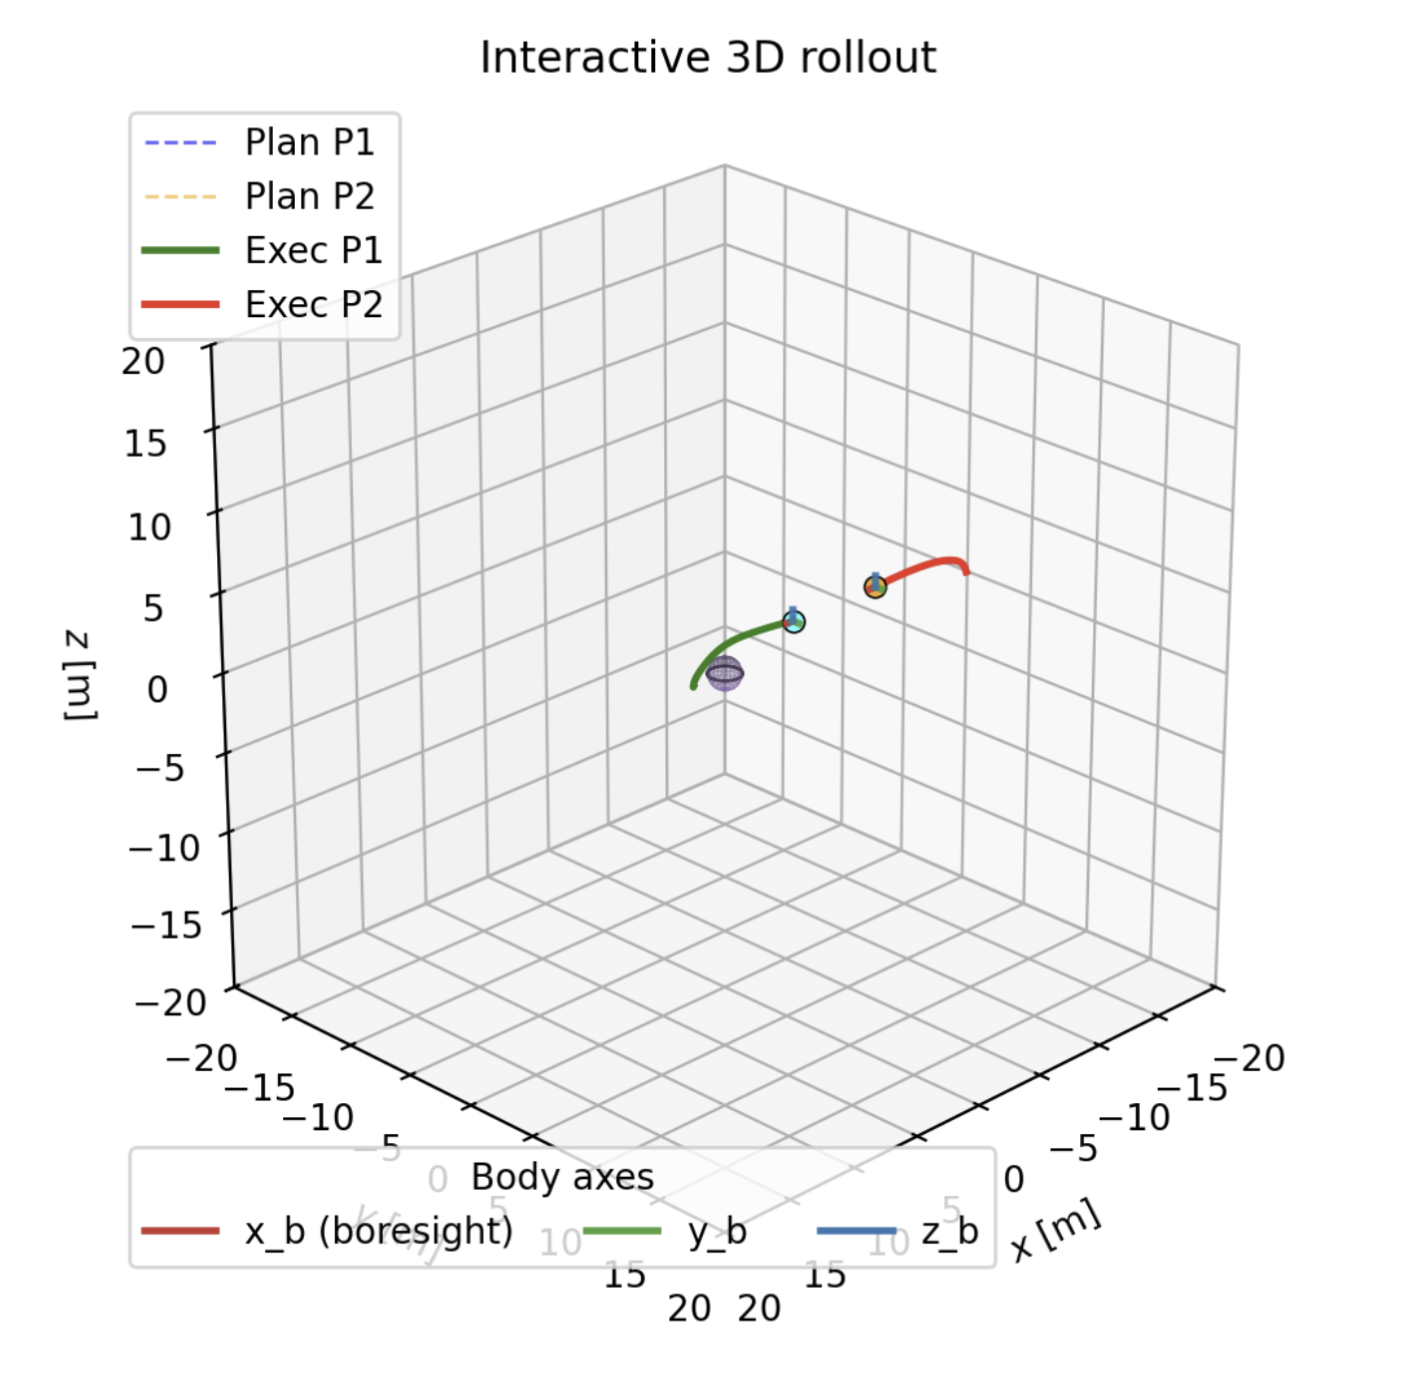
\includegraphics[width=\linewidth]{Figures/3D_Rollout.png}
    \end{minipage}
    % \hfill
    \begin{minipage}{0.45\linewidth}
        \centering
        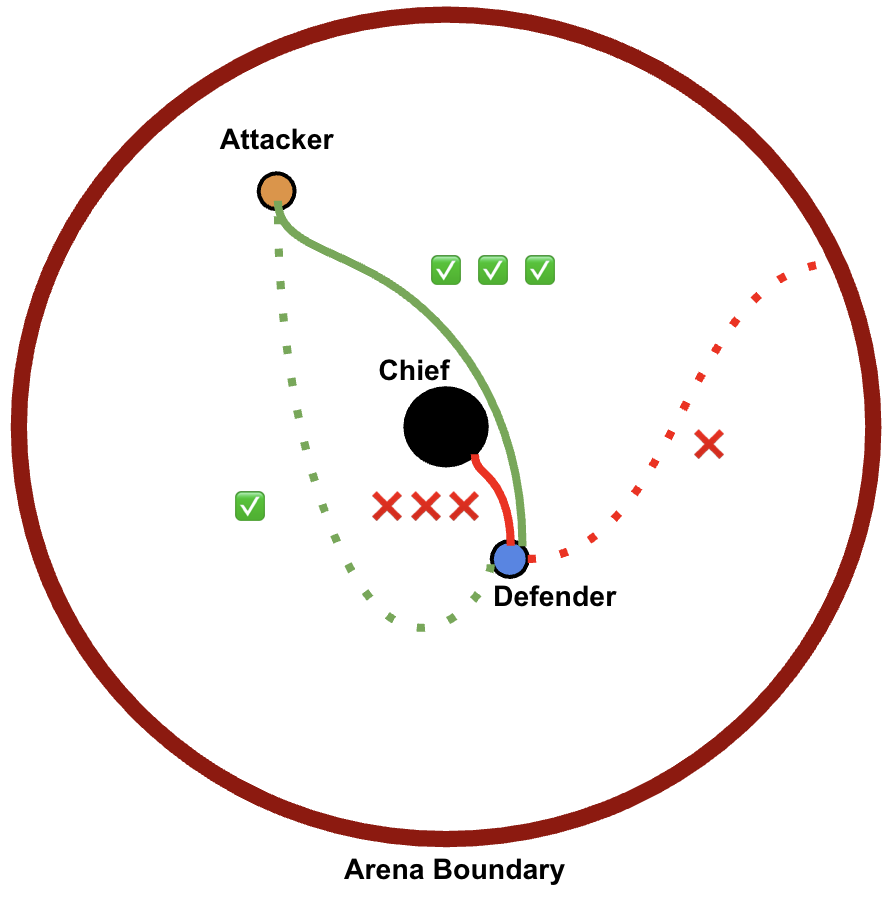
\includegraphics[width=\linewidth]{Figures/Training_Visualization.png}
    \end{minipage}
    \caption{Sample of a policy rollout showing the agents carrying the proposed zero-sum game setup (left), as well as a simple graphic describing training scenarios for the defender (right).}
    \label{fig:3D_Rollout_Double}
\end{figure}



%===========
\newpage


\section{\acs{hcw} (Hill--Clohessy--Wiltshire) orbital relative dynamics model}
\label{sec:dynamics-models}
\label{subsec:dynamics-hcw}

Based on the work by \cite{clohessy1960terminal} and \cite{hill1878researches}, we model the follower in the chief agent's Local Vertical, Local Horizontal (\acs{lvlh}) frame assuming a circular reference orbit of radius $r_0$ around a body with parameter $\mu$. The mean motion is defined as:
\[
n \;=\; \sqrt{\mu / r_0^3}
\]
Let $(x,y,z)$ be defined as the relative positions of the agents and let the control thrust acceleration of the agents be defined as:
$\mathbf{a} = [a_x, a_y, a_z]^\top$.
For small separations between agents and assuming the chief follows a circular orbit, the linearized \acs{hcw} equations are
\begin{align*}
\ddot{x} &= 2n \dot{y} + 3n^2 x  + a_x, \\
\ddot{y} &= - 2n \dot{x}            + a_y, \\
\ddot{z} &= - n^2 z                  + a_z
\end{align*}
Stacking the position and velocity elements into a single vector as 
$\mathbf{s} := [x\ y\ z\ \dot{x}\ \dot{y}\ \dot{z}]^\top$
gives the linear time invariant (\acs{lti}) form:
\begin{gather*}
\dot{\mathbf{s}} = F\mathbf{s} + G\mathbf{a},\\[4pt]
F =
\begin{bmatrix}
\mathbf{0}_{3\times3} & I_3\\[4pt]
\begin{array}{ccc}
3n^2 & 0   & 0\\
0    & 0   & 0\\
0    & 0   & -n^2
\end{array} &
\begin{array}{ccc}
0 & 2n & 0\\
-2n & 0 & 0\\
0 & 0 & 0
\end{array}
\end{bmatrix},
\quad
G =
\begin{bmatrix}
\mathbf{0}_{3\times3}\\[2pt]
I_3
\end{bmatrix}
\end{gather*}
With a sample time $\Delta t$, we do a zero order hold discretization as:
\begin{gather*}
A_d = e^{F\Delta t},\\[4pt]
B_d = \int_{0}^{\Delta t} e^{F\tau}\,G\,d\tau
\end{gather*}

From which we obtain our final dynamics evolution as:


\[
\mathbf{s}_{k+1} = A_d\mathbf{s}_k + B_d\mathbf{u}_k,
\qquad
A_d \in \mathbb{R}^{6\times 6},
\quad
B_d \in \mathbb{R}^{6\times 3}
\]


Note that \acs{hcw} is globally Linear Time Invariant (\acs{lti}) here only under certain assumptions, which are sufficient given the scope of this research: 

\begin{itemize}
    \item The chief agent is following a perfectly circular orbit with constant altitude. 
    \item We are dealing with small distances relative to the celestial object being orbited $\| (x,y,z)\| \ll r_0$
    \item The control accelerations exerted by the agents are small relative to the central gravitational field
\end{itemize}

These \acs{hcw} dynamics are used for all our trained policies and their respective evaluation described in this work.

In addition, we use elliptical dynamics only on the policy evaluation. Appendix~\ref{appendix:dynamics-elliptic-ltv} shows the derivation for these dynamics

\section{Orbits used in this work}
\label{subsec:dynamics-orbits-used}

Throughout this thesis, whenever we refer to \acs{hcw} and Elliptical dynamics we refer to just one chief orbit per dynamics model to exemplify each case within the context of the work. The commanded motion each agent undergoes then occurs relative to this chief orbit. The parameters of each of these orbits are:

\begin{table}[H]
\centering
\caption{Chief orbit parameters used for the \acs{hcw} and elliptic dynamics.}
\label{tab:chief-orbit-parameters}
\begin{tabular}{lcc}
\toprule
\textbf{Parameter} & \textbf{\acs{hcw} circular orbit} & \textbf{Elliptic orbit} \\
\midrule
Use case & Training and evaluation & Evaluation only \\
Radius / semi-major axis & $r_0 = 6771~\mathrm{km}$ & $a = 7646~\mathrm{km}$ \\
Eccentricity & $e = 0$ & $e = 0.0948$ \\
Perigee altitude & $400~\mathrm{km}$ & $550~\mathrm{km}$ \\
Apogee altitude & $400~\mathrm{km}$ & $2000~\mathrm{km}$ \\
Orbital period & $92.41~\mathrm{min}$ & $110.89~\mathrm{min}$ \\
\bottomrule
\end{tabular}
\end{table}

And the following is a visualization for these:

\begin{figure}[H]
    \centering
    
\includegraphics[width=0.8\linewidth]{Figures/Merged_Thesis/chief_orbit_hcw_vs_elliptic_ltv.png}
    \caption{Chief orbit geometry used for the \acs{hcw} and elliptic dynamics, showing the circular training/evaluation orbit and the elliptic evaluation-only orbit. Image credit: \acs{nasa}, Reid Wiseman, Artemis II (\cite{apod2026helloworld}).}
    \label{fig:Orbits_Visualization}
\end{figure}

\section{Full-State and Partial Observability Settings}

Note that this work also studies the proposed framework under two information settings: one with full-state observability and the other with partial observability. In the former, each agent has full-state access to its opponent. In the latter, each agent has to estimate its opponent's state via a bearings-only Extended Kalman Filter (\acs{ekf}), motivated by sensor limitations in real-life spacecraft applications. Studying both cases is meaningful as it allows us to compare performance under idealized conditions and under estimation-limited conditions. Therefore, we can use our findings to assess how the proposed framework degrades when moving toward more realistic sensor-based navigation settings.


\section{Assumptions}

Considering the problem that has been set up throughout this chapter, we will make a few assumptions throughout the remainder of this manuscript:



\begin{itemize}
    \item Both spacecraft agents are fully actuated and have continuous throttle control on each translational axis.
    \item The spacecraft used by both agents in the game are identical and have the same control parameters.
    \item Both agents follow the same dynamics model relative to the chief of the orbit.
    \item Attitude evolution is ignored throughout for the sake of simplicity: only translational motion is considered and in the \acs{ekf} setting the agents are considered to be facing each other at all times.
    \item The raw control actions from the learned policies are assumed to be realizable subject to the \acs{cbfqp} saturation filter.
    \item There is no actuator lag or delay across either spacecraft: the only lag present is the discrete $\Delta t$ timestep in the simulation.
    \item In the full-state setting of the game, each agent has access to its opponent's full state.
    \item Also in the full-state setting of the game, the orbital game is treated as a Markov Decision Process (\acs{mdp}) by both agents.
    \item In the partial-observability setting of the game, the opponent state is only obtained through bearings-only measurements.
    \item The defender and attacker remain within a bounded spherical arena during training and evaluation and, if they leave it, rollouts stop.
    \item Policies are trained with Hill-Clohessy-Wiltshire (\acs{hcw}) relative dynamics and are evaluated under both \acs{hcw} and elliptical linear time-varying relative dynamics.
    \item Sensor characteristics such as process noise, measurement noise, and randomized initial-condition dispersions are assumed to be adequately represented by the parameters chosen in the simulation.
    \item External environmental effects, such as atmospheric drag and solar wind, are ignored.
\end{itemize}
